% LaTeX source for textbook ``ThinkCPP , a game perspective''
% Copyright (C) 2023  Lisa Patacchiola, Allen B. Downey


\chapter{Conditionals}
\label{conditional}

\section{Floating-point}
\index{floating-point number}
\index{type!double}
\index{double (floating-point)}
\label{floating-point}

In the last chapter we had some problems dealing with numbers
that were not integers.  We worked around the problem by measuring
percentages instead of fractions, but a more general solution is
to use floating-point numbers, which can represent fractions
as well as integers.  In C++, there are two floating-point types,
called {\tt float} and {\tt double}.  In this book we will use
{\tt double}s exclusively.

You can create floating-point variables and assign values to them
using the same syntax we used for the other types.  For example:

\begin{lstlisting}
  double pi;
  pi = 3.14159;
\end{lstlisting}
%
Remember, it is also legal to declare a variable and assign a value to it at the
same time:

\begin{lstlisting}
  int x = 1;
  string empty = "";
  double pi = 3.14159;
\end{lstlisting}
%
In fact, this syntax is quite common.  A combined declaration
and assignment is sometimes called an {\bf initialization}.

\index{initialization}
(FYI, if you are using C++20, you can use the mathematical
constant of PI, like the following:
\begin{lstlisting}
  double mypi = std::numbers::pi;
\end{lstlisting}
There are lots of constants available. We will be talking 
more about them when we talk about the Math library in Section \ref{mathlibrary}.)


Although floating-point numbers are useful, they are
often a source of confusion because there seems to be an
overlap between integers and floating-point numbers.  For
example, if you have the value {\tt 1}, is that an integer,
a floating-point number, or both?

Strictly speaking, C++ distinguishes the integer value {\tt 1}
from the floating-point value {\tt 1.0}, even though they
seem to be the same number.  They belong to
different types, and strictly speaking, you are not allowed
to make assignments between types.  For example, the following
is illegal

\begin{lstlisting}
    int checkMe = 1.1;  // WARNING!
\end{lstlisting}
%
because the variable on the left is an {\tt int}
and the value on the right is a {\tt double}. If you are
using the legacy initialization (see above), the compiler
will give you a warning and let you know that checkMe will
be set to 1, and not 1.1. But, your code will continue to
run. If you want an error to happen 
instead, you can use the braced initialization:
\begin{lstlisting}
    int checkMe{1.1};   // ERROR!
\end{lstlisting}
Instead of giving a warning, the compiler will create an
an error, complaining "type 'double' cannot be narrowed to 'int' in initializer list". 
\index{braced initialization}
\index{initialization!braced}

But it is easy
to forget this "no assignment between types" rule, especially because there are places where C++
automatically converts from one type to another.
For example,

\begin{lstlisting}
    double y = 1;
\end{lstlisting}
%
should technically not be legal, but C++ allows it by converting the
{\tt int} to a {\tt double} automatically.  This leniency is
convenient, but it can cause problems; for example:

\begin{lstlisting}
    double y = 1 / 3;
\end{lstlisting}
%
You might expect the variable {\tt y} to be given the value
{\tt 0.333333}, which is a legal floating-point value, but in
fact it will get the value {\tt 0.0}.  The reason is that the
expression on the right appears to be the ratio of two integers,
so C++ does {\em integer} division, which yields the integer
value {\tt 0}.  Converted to floating-point, the result is
{\tt 0.0}.

One way to solve this problem (once you figure out what
it is) is to make the right-hand side a floating-point
expression:

\begin{lstlisting}
    double y = 1.0 / 3.0;
\end{lstlisting}
%
This sets {\tt y} to {\tt 0.333333}, as expected.

\index{arithmetic!floating-point}

All the operations we have seen---addition, subtraction,
multiplication, and division---work on floating-point values,
although you might be interested to know that the underlying mechanism
is completely different.  In fact, most processors have special
hardware just for performing floating-point operations.

\subsection{Converting from {\tt double} to {\tt int}}
\label{rounding}
\index{rounding}
\index{typecasting}
\index{static cast}
\index{cast!static}

As I mentioned, C++ converts {\tt int}s
to {\tt double}s automatically if necessary, because no
information is lost in the translation.  On the other hand,
going from a {\tt double} to an {\tt int} requires rounding
off.  C++ doesn't perform this operation automatically, in
order to make sure that you, as the programmer, are aware
of the loss of the fractional part of the number.

The simplest way to convert a floating-point value to an integer is to
use a {\bf typecast}.  Typecasting is so called because it allows you
to take a value that belongs to one type and ``cast'' it into another
type (in the sense of molding or reforming, not throwing).

The syntax for typecasting is different than code we have seen so far.  For example:

\begin{lstlisting}
  double pi = 3.14159;
  int x = static_cast<int>(pi);
\end{lstlisting}
%
The {\tt static\_cast<int>} casting operator returns an integer, so {\tt x} gets the value
3.  Converting to an integer always rounds down, even if the fraction
part is 0.99999999.

For every type in C++, there is a corresponding function that
typecasts its argument to the appropriate type. The format follows the following pattern:

\begin{lstlisting}
  T newVariable = static_cast<T>(oldVariable);
\end{lstlisting}
To use this, change T to be the type you are converting into. Put the variable name you are converting where "oldVariable" is. Last, change "newVariable" to the name of the variable you want the new value to be placed. 

Here are some examples so you can try them out: \url{https://replit.com/@lpatacch/DivisionDoubleIntExamples#divdoubles.cpp }

\section{Conditional execution}
\index{conditional}
\index{statement!conditional}
\index{if}

In order to write useful programs, we almost always need the ability to check certain conditions and change the behavior of the program accordingly.  {\bf Conditional statements} give us this ability.  The simplest form is the {\tt if} statement:

\begin{lstlisting}
  if (x > 0) {
    std::cout << "x is positive" << std::endl;
  }
\end{lstlisting}
%
That code is doing the following:
\begin{verbatim}
IF x is greater than 0 THEN
    Output "x is positive" and then go to the next line
ENDIF
\end{verbatim}
That also means that if x is zero or less, it will not output anything and just go to the following line of code. 

The expression in parentheses is called the condition.
If it is true, then the statements in brackets get executed.
If the condition is not true, nothing happens.

\begin{figure}[h]
    \centering
    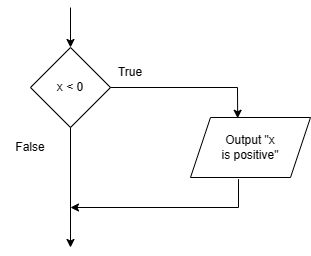
\includegraphics[height=6cm]{images/ifflow.png}
    \caption{If flowchart}
    \label{fig:ifflow}
\end{figure}

\index{operator!comparison}
\index{comparison!operator}

The condition can contain any of the {\tt comparison operators}:

\begin{lstlisting}
    x == y           // x equals y
    x != y           // x is not equal to y
    x > y            // x is greater than y
    x < y            // x is less than y
    x >= y           // x is greater than or equal to y
    x <= y           // x is less than or equal to y
\end{lstlisting}
%
Although these operations are probably familiar to you, the
syntax C++ uses is a little different from mathematical
symbols like $=$, $\neq$ and $\le$.  A common error is
to use a single {\tt =} instead of a double {\tt ==}.  Remember
that {\tt =} is the assignment operator, and {\tt ==} is
a comparison operator.  Also, there is no such thing as
{\tt =<} or {\tt =>}.

Unfortunately, the default behavior in many compilers is to not display warnings when you use one equal instead of two in an if statements. (Check out Chapter \ref{showwarning} if you want to know how to turn on the warnings.) Be sure to be careful when you are using equal signs and if statements.

The two sides of a condition operator have to be the same
type.  You can only compare {\tt ints} to {\tt ints} and
{\tt doubles} to {\tt doubles}. 

\section {Alternative execution}
\label{alternative}
\index{conditional!alternative}
\index{if else}
\index{else}

A second form of conditional execution is alternative execution,
in which there are two possibilities, and the condition determines
which one gets executed.  This is sometimes called the {\tt if else} statement. The syntax looks like:

\begin{lstlisting}
    
  if (x%2 == 0) {
    std::cout << "x is even" << std::endl;
  } else {
    std::cout << "x is odd" << std::endl;
  }
\end{lstlisting}
%
(If you do not remember what the \% sign is doing, check out the
Modulus section in Chapter~\ref{modulus})
That code is doing the following:
\begin{verbatim}
IF x mod 2 is equal to 0 THEN
    Output "x is even" and then go to the next line
ELSE
    Output "x is odd" and then go to the next line
ENDIF
\end{verbatim}
If the remainder when {\tt x} is divided by 2 is zero, then
we know that {\tt x} is even, and this code displays a message
to that effect.  If the condition is false, the second
set of statements is executed.  Since the condition must
be true or false, exactly one of the alternatives will be
executed.

\begin{figure}[h]
    \centering
    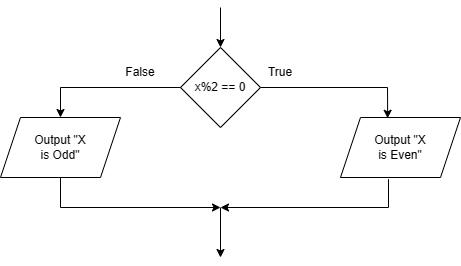
\includegraphics[height=6cm]{images/ifelseflow.png}
    \caption{If else flowchart}
    \label{fig:ifelseflow}
\end{figure}


\section {Chained conditionals}
\index{conditional!chained}

Sometimes you want to check for a number of related conditions
and choose one of several actions.  One way to do this is by
{\bf chaining} a series of {\tt if}s and {\tt else}s:

\begin{lstlisting}
  if (x > 0) {
    std::cout << "x is positive" << std::endl;
  } else if (x < 0) {
    std::cout << "x is negative" << std::endl;
  } else {
    std::cout << "x is zero" << std::endl;
  }
\end{lstlisting}
%
These chains can be as long as you want, although they can
be difficult to read if they get out of hand.  One way to
make them easier to read is to use standard indentation,
as demonstrated in these examples.  If you keep all the
statements and squiggly-braces lined up, you are less
likely to make syntax errors and you can find them more
quickly if you do.

\section{Nested conditionals}
\index{conditional!nested}

In addition to chaining, you can also nest one conditional
within another.  We could have written the previous example
as:

\begin{lstlisting}
  
  if (x == 0) {
    std::cout << "x is zero" << std::endl;
  } else {
    if (x > 0) {
      std::cout << "x is positive" << std::endl;
    } else {
      std::cout << "x is negative" << std::endl;
    }
  }
\end{lstlisting}
%
There is now an outer conditional that contains two branches.  The
first branch contains a simple output statement, but the second
branch contains another {\tt if} statement, which has two branches
of its own.  Fortunately, those two branches are both output
statements, although they could have been conditional statements as
well.
\begin{verbatim}
    IF x is equal to zero THEN
        Output "X is zero"
    ELSE 
        IF x is greater than zero THEN
            Output "x is positive"
        ELSE 
            Output "x is negative"
        ENDIF
    ENDIF
\end{verbatim}
\begin{figure}[h]
    \centering
    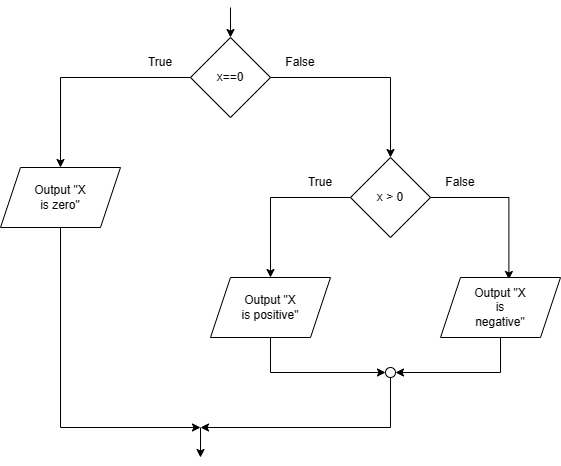
\includegraphics[height=6cm]{images/nestedifflow.png}
    \caption{Nested if/else statement}
    \label{fig:nestedifelse}
\end{figure}
Notice again that indentation helps make the structure
apparent, but nevertheless, nested conditionals get difficult to read
very quickly.  In general, it is a good idea to avoid them when you
can.

\index{nested structure}

On the other hand, this kind of {\bf nested structure} is common, and
we will see it again, so you better get used to it.

\section{Logical operators}
\index{logical operator}
\index{operator!logical}
Nested if statements can get tricky to look at, so there are a couple of different ways to make it look less complex. The first we will look at is "logical operators".
There are three {\bf logical operators} in C++: AND, OR and NOT,
which are denoted by the symbols {\tt \&\&}, {\tt ||} and
{\tt !}.  The semantics (meaning) of these operators is similar
to their meaning in English.  For example {\tt x > 0 \&\& x < 10}
is true only if {\tt x} is greater than zero AND less than 10.

\index{semantics}

{\tt n\%2==0 || n\%3 == 0} is true if {\em either} of
the conditions is true, that is, if the number is divisible by 2 OR the
number is divisible by 3.

Finally, the NOT operator has the effect of negating or
inverting a bool expression, so {\tt !(n\%2 == 0)} is true
if {\tt (n\%2 == 0)} is false; that is, if the number is odd.

\index{nested structure}

Logical operators often provide a way to simplify nested
conditional statements.  For example, how would you write
the following code using a single conditional?

\begin{lstlisting}
  
  if (x > 0) {
    if (x < 10) {
      std::cout << "x is a positive single digit.";
      std::cout << std::endl;
    }
  }
\end{lstlisting}

But, you need to be careful when you are making a comparison. What makes sense to a human does not make sense to a computer. If you want to see if x is less than y and z, the following are what many students think is a solution (it is not.)

\begin{lstlisting}

if ((x < y) && (z))   // WRONG!
{
}
\end{lstlisting}
Although it is comparing x to y, it is not comparing z. It is just checking if Z is zero or not. Instead, this is what the if statement should be:
\begin{lstlisting}
if ((x < y) && (x < z))  // this is the way!  
\end{lstlisting}


\section{Short circuiting the logic}
If you are not exactly sure how AND works, here is a table that explains the specifics. If you have one comparison (first) and it is ANDed to the second comparison (second), the third column is the result.
\begin{table}[h]
\centering
\begin{tabular}{ | c | c | c | }
\hline
 first & second & first \&\& second \\\hline
 true & true & true \\ 
 true & false & false \\  
 false & true & false \\
 false & false & false \\
\hline
\end{tabular}
    \caption{Truth table for AND}
    \label{tab:andtruth}
\end{table}

If you take a look at the table, you may notice that the only way the final result is true is that both comparisons need to be true. Because of that, when C++ code is running, it has a shortcut. If it notices the first item of an AND comparison is false, it does not bother checking the second comparison. If you happen to know the comparison that is false more often, you can have your code run faster by having it be the first of the comparisons.

Next is how the OR comparison works. If you look at the OR truth table, you will notice that you only need one item to be true for the result to be true.
\vspace{0.1in}
\begin{table}[h]
\centering
\begin{tabular}{ | c | c | c | }
\hline
 first & second & first OR second \\\hline
 true & true & true \\ 
 true & false & true \\  
 false & true & true \\
 false & false & false \\
\hline
\end{tabular}
    \caption{Truth table for OR}
    \label{tab:ortruth}
\end{table}
\vspace{0.1in}
Just like the AND comparison, there is a shortcut. As soon as it sees a "true", the program goes straight to the resulting code. If you know the comparison that happens to be true more often, you can have your code run quicker by having it be the first comparison.

\section{Conditional Operator}
\index{conditional operator}
\index{operator!conditional}
There is another operator that people can use instead of the 
if/else statements. It is a more compact way to check a condition,
and then set the appropriate value. For example:
\begin{lstlisting}
  y = ( x < 0 ) ? -1 : 1;
\end{lstlisting}
That line is equivalent to:
\begin{lstlisting}
  if ( x < 0 ) {
    y = -1;
  }
  else {
    y = 1;
  }
\end{lstlisting}
It can also be used to decide what to print:
\begin{lstlisting}
  std::cout << ((w < 0)? "negative":"positive or zero");
\end{lstlisting}
The above code checks what w is set to. If it is less than 0, it 
will print "negative". Otherwise, it prints "positive or zero".
\section{{\tt switch} statement}
\index{switch statement}
\index{statement!switch}
\label{switch}

Another method that we can use instead of a complex if statement is {\tt switch}
statements.  A {\tt switch} statement
is an alternative to a chained conditional that is syntactically
prettier and often more efficient.  It looks like this:

\begin{lstlisting}
  
 switch (symbol) {
  case '+':
    z = x + y;
    break;
  case '*':
    z = x * y;
    break;
  default:
    std::cout << "I only know how to perform addition";
    std::cout <<" and multiplication" << std::endl;
    break;
 }
\end{lstlisting}
%
This {\tt switch} statement is equivalent to the following chained
conditional:

\begin{lstlisting}
  
  if (symbol == '+') {
    z = x + y;
  } else if (symbol == '*') {
    z = x * y;
  } else {
    std::cout << "I only know how to perform addition";
    std::cout << "and multiplication" << std::endl;
  }
\end{lstlisting}
%
In general it is good style to include a {\tt default} case in
every {\tt switch} statement, to handle errors or unexpected values.
\index{default}

The {\tt break} statements are necessary in each branch
in a {\tt switch} statement because otherwise the flow of execution
``falls through'' to the next case.  Without the {\tt break} statements,
the symbol {\tt +} would make the program perform addition, and
then perform multiplication, and then print the error message.
Occasionally this feature is useful, but most of the time it is
a source of errors when people forget the {\tt break} statements.

\index{break statement}
\index{statement!break}

\subsection{Fallthrough}
Here is an example of code using switch that is using the fall through feature. This method of stacking cases is common, so no error message is created if the compiler sees this:
\begin{lstlisting}
  /* In this code, the user types a character to decide 
     which way to go. If they type 'L' or 'l', they will 
     go left. If they type 'R' or 'r', they will go 
     right. If they type anything else, there is an 
     error message
   */
   
  switch (direction) {
    case 'L':
    case 'l':
        std::cout << "Going left" << std::endl;
        break;
    case 'R':
    case 'r':
        std::cout << "Going Right" << std::endl;
        break;    
    default:
        std::cout << "Please choose R or L" << std::endl;
  }
\end{lstlisting}
The above code allows the programmer to have the same result if 
a person typed either R or r. 

The next example is something more uncommon. It is using the fallthrough feature without stacking cases. Each case will be
printing something connected to its case, and then an printing the items for the lower cases.

\begin{lstlisting}
  std::cin >> dayOfChristmas;
  std::cout << "On the " << dayOfChristmas;
  std::cout << " day of Christmas";
  std::cout << " my true love gave to me";
  switch (dayOfChristmas) {
    case 3:
        std::cout << " 3 french hens,";
    case 2:
        std::cout << " 2 calling birds, and";
    case 1:
        std::cout << " a partridge in a pear tree";
        std::cout << std::endl;
  }
\end{lstlisting}

There is more of a chance that this type of code is a mistake, so the C++ 2017 standard (and the later standards) now has a warning if you write a switch statement with this feature. If you want to avoid this warning, you can add the following:
\begin{verbatim}
    [[fallthrough]];    
\end{verbatim}
where a "break" statement would normally be. So, if you take the previous example, it would look like this:
\begin{lstlisting}
  std::cout << "On the " << dayOfChristmas;
  std::cout << " day of Christmas";
  std::cout << " my true love gave to me";
  switch (dayOfChristmas) {
    case 3:
        std::cout << " 3 french hens,";
        [[fallthrough]];
    case 2:
        std::cout << " 2 calling birds, and";
        [[fallthrough]];
    case 1:
        std::cout << " a partridge in a pear tree";
        std::cout << std::endl;
    }
\end{lstlisting}

Remember, this warning removal feature is ONLY available if you are using the 2017 standard or later. (For information on how to change the standard on Reddit, check out Section \ref{changestandard}.)

\section{Pseudocode}
\index{pseudocode}
FIXME
One important point is to not make your pseudocode too technical. You are not trying to write the code itself, just a plan on how the code could be written.

\section{Flowcharts}
\index{flowchart}
Just like pseudocode, I have put a few figure of flowcharts around the if and if else statements. Flowcharts are another way to show how code is running. Instead of using just words, flowcharts add shapes and arrows to help people understand the logic of the code. There are some specifics of how flowcharts generally work.

FIXME
\subsection{shapes}
selection (if statements)
processing (math)
input and output
Start/Stop
part of a large algorithm start/stop
\subsection{How they connect}
Each section is a component and it should not jump from one section to another
"spaghetti code"
Picture of a flowchart with the improper shared middle section

\section{Testing Techniques}
Now that we have code with if statements, we can't just run the 
code once to make sure it works. To be truly sure that the entire
program works, it is important to test each possible path of the
program. For example, if we have a program that checks to see if
a number is less than zero, we should check a negative number, 
a positive number, and zero to make sure the program works. 

\begin{lstlisting}
int main() {
  int x = 1; // Later, set to 0, and then -1.
  if (x == 0) {
    std::cout << "x is zero" << std::endl;
  } else {
    if (x > 0) {
      std::cout << "x is positive" << std::endl;
    } else {
      std::cout << "x is negative" << std::endl;
    }
  }
}
\end{lstlisting}
If I put those values in, I should see the x is zero for zero, x is
positive for the 1, and x is negative for the -1. If one of those does not print the correct item, I would know there is a bug, and 
would know where to check. For example, if the "x is zero" did not print, I would be looking at the first if statement condition. Check
the paths in Figure \ref{fig:nestedpath}.

\begin{figure}[h]
    \centering
    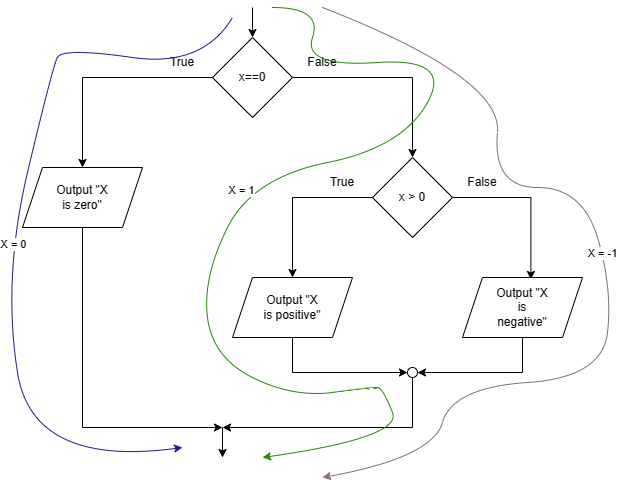
\includegraphics[width=9cm]{images/nestedifflow - Path.png}
    \caption{Nested if else flowchart with pathlines}
    \label{fig:nestedpath}
\end{figure}
It is good to test each section of code before adding more code
to the program. This will allow you to have a better idea where the
bug could be.

\section{Exercises}
\subsection{Rock Paper Scissors}
FIXME
\subsection{Magic 8 Ball}
FIXME
\subsection{Decision Maker}
FIXME
This assignment will be based on the assignment below.
Students are asked to create a formula that makes a judgement
But, should they make a judgement without talking to others?

%https://docs.google.com/document/d/1t_ZvI0brEiHdb4CvvjA5X7-uUSU56p9h7alAf3RAcbg/edit# 

\section{Glossary}

\begin{description}
\item[floating-point:] A type of variable (or value) that can contain
fractions as well as integers.  There are a few floating-point types
in C++; the one we use in this book is {\tt double}.

\item[conditional:]  A block of statements that may or may not
be executed depending on some condition.

\item[chaining:]  A way of joining several conditional statements
in sequence.

\item[nesting:] Putting a conditional statement inside one or both
branches of another conditional statement.

\item[switch statement:] A different way to write conditional code. The switch selects the case to run depending on the variable it is checking.

\item[pseudocode:]  A way of designing programs by writing
rough drafts in a combination of keywords and English.

\item[flowchart:] A way of designing programs with shapes and arrows used to show the flow of the program. 

\index{conditional}
\index{conditional!chained}
\index{conditional!nested}
\index{floating-point}
\index{switch statement}
\index{pseudocode}
\index{flowchart}

\end{description}


